
\section{Shape modeling and synthesis}
\label{sec:modeling}

So far, the creation of detailed three-dimensional content remains a tedious task which can mainly be performed by skilled artists.
3D content creation has been a major bottleneck hindering the development of ubiquitous 3D graphics.
Thus, providing easy-to-use tools for casual and novice users to design and create 3D models has been a key
challenge in computer graphics. To address this challenge, current literature has been focused on two main directions, i.e.,
intelligent interfaces for interactive shape modeling and smart models for automated model synthesis.
%The former strives to endow a modeling interface with a higher-level understanding of the structure and semantics of 3D shapes, allowing the interface to reason around the incomplete shape being modeled~\cite{Chaudhuri:2010:DDS}.
%
%The second direction follows the modeling-by-example paradigm~\cite{Funkhouser:2004:MBE}.
%The second direction follows the by-example synthesis paradigm.
%Given a set of semantically related shapes, the goal is to generate more shapes which are both novel and plausible.
%This can be approached by several models, such as generative models~\cite{Allen:2003:SHB},
%evolutionary computation~\cite{Sims:1991:AE}, and inverse procedural modeling~\cite{Stava:2010:IPM}.
The former strives to endow modeling interfaces with a higher-level understanding of the structure and semantics
of 3D shapes, allowing the interface to reason around the incomplete shapes being modeled. The latter direction focuses on developing data-driven models to synthesize new shapes automatically.
%The core problem is to learn from the input shape set a model that encapsulates
%geometric, structural and functional constraints to drive the automatic synthesis of novel shapes.
The core problem is to learn generative shape models from a set of exemplars (e.g., probability distributions, fitness functions, functional constraints, etc) so that the synthesized shapes are plausible and novel.
It can be seen that both of the two paradigms depend on data-driven modeling of shape structures and semantics.
With the availability of large 3D shape collections, the data-driven approach becomes a promising answer to the content creation bottleneck.

\subsection{Interactive shape modeling and editing}
\label{sec:interactive_modeling}
%Interactive modeling is perhaps the most prevailing manner of designing and creating 3D models, as
%reflected by the highly matured modeling softwares (3DS Max, Maya, etc.).
Interactive 3D modeling software (3DS Max, Maya, etc.) provide artists with a large set of tools
for creating and editing detailed 3D models.  Unfortunately, this same software is often onerous to harness for non-professional users.
For casual users, more intuitive modeling interfaces with a certain machine intelligence are to be preferred. Below, we discuss such methods for assembly-based modeling and guided shape editing.

%\vangelis{it is ok, we discuss this high-level understanding many times in the text already}
%The key to making interactive modeling more accessible is to equip the interfaces with a higher-level understanding of the structure and semantics of 3D shapes, so that they can reason about the partially modeled shapes, to enhance the modeling process with useful suggestions, informative guidance and smart automation.

\paragraph*{Assembly-based modeling.}
Early works on 3D modeling based on shape sets are primarily driven by the purpose of \emph{content reuse}
in part-assembly based modeling approaches.
The seminal work of modeling by example~\cite{Funkhouser:2004:MBE} presents a pioneering system
of shape modeling by searching a shape database for parts to reuse in the construction of new shapes.
Kraevoy et al.~\shortcite{Kreavoy:2007:MIC} describe a system for shape creation
via interchanging parts between a small set of compatible shapes.
Guo et al.~\cite{Guo:2014:CG} propose assembly-based creature modeling guided by a shape grammar.

\rev{Beyond content reuse through database queries or hand-crafted rules, Chaudhuri and Koltun~\shortcite{Chaudhuri:2010:DDS} propose a data-driven technique
for suggesting the modeler with shape parts that can potentially augment the current shape being built.}
Such part suggestions are generated through retrieving a shape from a database based on partial shape matching.
Although this is a purely geometric method without accounting for the semantics of shape parts,
it represents the first attempt at utilizing a shape database to \emph{augment the modeling interface}.
Later, Chaudhuri et al.~\shortcite{Chaudhuri:2011:prabm} show that the incorporation of
semantic relationships increases the relevance of presented parts.
Given a repository of 3D shapes, the method learns a probabilistic graphical model encoding semantic and geometric
relationships among shape parts. During modeling, inference in the learned Bayesian network
is performed to produce a relevance ranking of the parts.

A common limitation of the above techniques is that they do not provide a way to directly express a high-level design goal (e.g. ``create a cute toy''). Chaudhuri et al.~\shortcite{Chaudhuri:2013:ACC} proposed a method that learns semantic attributes for shape parts that reflect the high-level intent people may have for creating content in a domain (e.g. adjectives such as ``dangerous'', ``scary'' or ``strong'') and ranks them according to the strength of each learned attribute (Figure \ref{fig:attribit}). During an interactive session, the user explores and modifies the strengths of semantic attributes to generate new part assemblies.

3D shape collections can supply other useful information as well, such as contextual and spatial relationships between shape parts,
to enhance a variety of modeling interfaces.
Xie et al.~\cite{Xie:2013:S2D} propose a data-driven sketch-based 3D modeling system.
In the off-line learning stage, a shape database is pre-analyzed to extract the contextual information among parts.
During the online stage, the user designs a 3D model by progressively sketching its parts and retrieving and assembling
shape parts from the database. Both the retrieval and assembly are assisted by
precomputed contextual information so that more relevant parts can be returned and selected parts can be automatically placed.
Inspired by the ShadowDraw system~\cite{Lee:2011:SD}, Fan et al.~\cite{Fan:2013:MBD} propose 3D modeling by drawing with
data-driven shadow guidance. The user's strokes are used to query a 3D shape database for generating the shadow image,
which in turn can guide the user's drawing. Along the drawing, 3D candidate parts are retrieved for assembly-based modeling.
\fix{
Starting from a collection of expertly-created, fabricable 3D models, Schulz et al.~\cite{Schulz:2014:DFE} extract
parameterized design templates encoding all information necessary for fabrication.
The templates can then be used to generate new fabricable models in an interactive design system.
}


\paragraph*{Shape editing.}
The general idea of data-driven shape editing is to learn a model from a collection of closely related shapes
that characterizes the plausible variations or deformations of the shapes in this collection.  In this way, the learned model
can be used to constrain a user's edit to maintain plausibility.
For organic shapes, such as human faces~\cite{Blanz:1999:MMS,Chen:2014:FED} or bodies~\cite{Allen:2003:SHB},
parametric models can be learned from a shape set characterizing its shape space.
Such parametric models can be used to edit the shapes through exploring the shape space with the set of parameters.

%For man-made shapes, however, learning such parametric shape space is intractable since their plausibility is related with structure~\cite{Mitra:2014:SASP}.
% \vangelis{structure can be parametrized as well}
An alternative widely-adopted approach is the analyze-and-edit paradigm.  This technique first extracts the structure of the input shape, and then uses this structure to constrain the editing phase to be more tenable~\cite{Gal:2009:IAA}.
Instead of learning structure from a single shape, Fish et al.~\cite{Fish:2014:MR} learn it from a set of shapes that belong to the same family, resulting in a set of probability distributions characterizing the part arrangements. These distributions can be used to guide structure-preserving editing, where models can be
edited while maintaining their familial traits.
Yumer et al.~\cite{Yumer:2014:CCH} extract co-constrained handles from a set of shapes for shape deformation.
The handles are generated based on co-abstraction~\cite{Yumer:2012:CSC} of the set of shapes and the deformation co-constraints are learned statistically from the set. \rev{The deformation handles can also be controlled with continuous semantic attributes \cite{Yumer:2015:SSE}.} \revnew{This approach also benefit from deep neural network trained to predict appropriate deformations for 3D models~\cite{yumer2016learning}.}

Based on learned structures from a database of 3D models, Xu et al.~\cite{Xu:2011:PMO} propose photo-inspired 3D object modeling.
Guided by the object in a photograph, the method creates a 3D model as a geometric variation of a candidate model retrieved from the database.
Due to the pre-analyzed structural information, the method addresses the ill-posed problem of 3D modeling from a single 2D image
via structure-preserving 3D warping. The final result is structurally plausible and is readily usable for subsequent editing.
Moreover, the resulting 3D model, although built from a single view, is structurally coherent from all views.

\subsection{Automated synthesis of shapes}
\label{sec:synthesis}
\begin{figure}[t]
\centering
    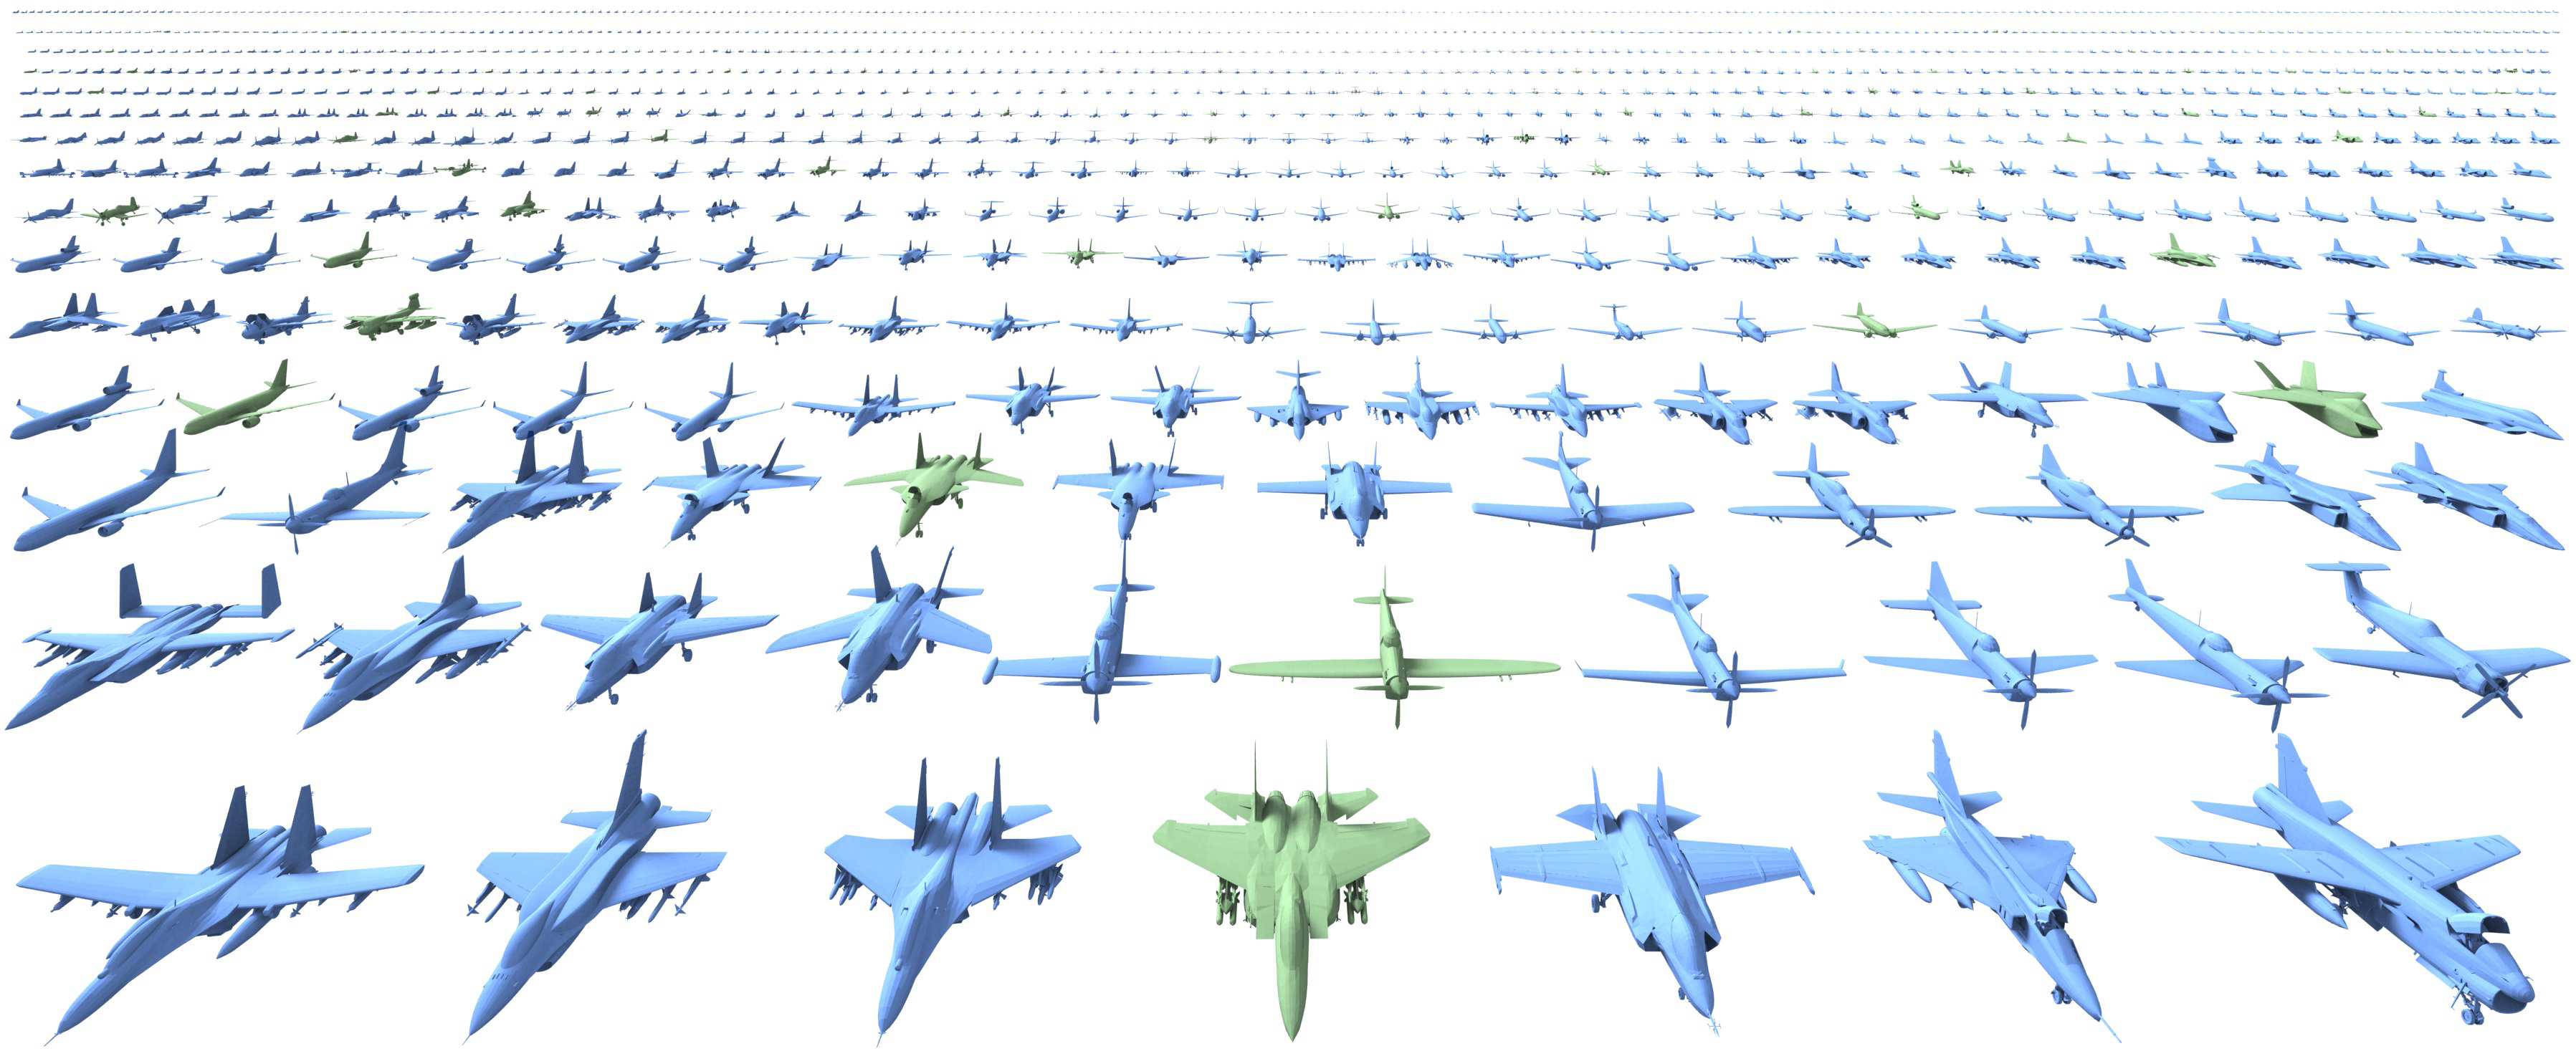
\includegraphics[width=.95\columnwidth]{fig/img/kalogerakis_sig12_synthesis}
    %\vspace{-0.3cm}
    \caption{
Given a hundred training airplanes (in green), the probabilistic model from \cite{Kalogerakis:2012:PMC} synthesizes several hundreds of new airplanes (in blue).}
    \label{fig:kalogerakis_sig12_synthesis}
\end{figure}



\rev{Many applications such as 3D games and films require large collections of 3D shapes for populating their environments. Modeling each shape individually can be tedious even with the best interactive tools. The goal of data-driven shape synthesis algorithms is to generate several shapes automatically with no or very little user supervision: users may only provide some preferences or high-level specifications to control the shape synthesis process. Existing methods achieve this task by using probabilistic generative models of shapes, evolutionary methods, or learned probabilistic grammars.}

\paragraph*{Statistical models of shapes.} The basic idea of these methods is to define a parametric shape space and then fit a probability distribution to the data points that represent the input exemplar shapes. Since the input shapes are assumed to be plausible and desired representatives of the shape space, high-probability areas of the shape space which tend to become associated with new, plausible shape variants. \rev{ This idea was first explored in the context of parametric models \cite{Blanz:1999:MMS,Allen:2003:SHB}, discussed in Section \ref{sec:recon}. By associating each principal component of the shape space defined by these methods with a Gaussian distribution, this distribution can be sampled to generate new human faces or bodies (Figure \ref{fig:allen_sig03_human}). Since the probability distribution of plausible shapes tends to be highly non-uniform in several shape classes, Talton et al. \cite{Talton:2009:EMC} use kernel density estimation with Gaussian kernels to represent plausible shape variability. The method is able to generate new shapes for tree and human body parametric spaces. }

Shapes have structure i.e., shapes vary in terms of their type and style, different shape styles have different number and type of parts, parts have various sub-parts that can be made of patches, and so on. Thus, to generate shapes in complex domains, it is important to define shape spaces over structural and geometric parameters, and capture hierarchical relationships between these parameters at different levels. Kalogerakis et al. \cite{Kalogerakis:2012:PMC} (Figure \ref{fig:kalogerakis_sig12_synthesis}) proposed a probabilistic model that represents variation and relationships of geometric descriptors and adjacency features for different part styles, as well as variation and relationships of part styles and repetitions for different shape styles. The method learns the model from a set of consistently segmented shapes. Part and shape styles are discovered based on latent variables that capture the underlying modes of shape variability. The method uses a search procedure to assemble new shapes from parts of the input shapes according to the learned probability distribution. Users can also set preferences for generating shapes from a particular shape style, with given part styles or specific parts. \fix{Instead of relying on pre-segmented shapes and high-level part descriptors to encode shape variability, Huang et al. \cite{Huang:2015:AS3} propose a probabilistic model that jointly estimates shape segmentation, surface correspondences, and surface descriptors from an input shape dataset. A deep learning procedure was used to capture hierarchical relationships of corresponding surface point positions and parts as well as their existence in the input shapes. Their probabilistic model can be sampled to directly generate point-sampled surface geometry and shape structure.}

\paragraph*{Set evolution.} \rev{Xu et al. \cite{Xu:FDS:2012} developed a method for generating shapes inspired by the theory of evolution in biology.} The basic idea of set evolution is to define cross-over and mutation operators on shapes to perform part warping and part replacement. Starting from an initial generation of shapes with part correspondences and built-in structural information such as inter-part symmetries, these operators are applied to create a new generation of shapes. A selected subset from the generation is presented via a gallery to the user who provides feedback to the system by rating them. The ratings are used to define the fitness function for the evolution. Through the evolution, the set is personalized and populated with shapes that better fit to the user. At the same time, the system explicitly maintains the diversity of the population so as to prevent it from converging into an ``elite'' set.

\paragraph*{Learned shape grammars.} Talton et al. \cite{Talton:2012:LDP} leverage techniques
from natural language processing to learn probabilistic generative grammars of shapes. The method takes as input a set of exemplar shapes represented with a scene graph specifying parent/child relationships and
relative transformations between labeled shape components. They use Bayesian inference to learn a probabilistic formal grammar that can be used to synthesize novel shapes. 

